\documentclass{beamer}
\usepackage{tabularx}
\usepackage{booktabs}
\usepackage{csquotes}
% Include Graphic-files:
\usepackage{graphicx}
\usepackage{caption}
\usepackage{subfig}
\usepackage{url}
%\usepackage{subfig}
\newsubfloat{figure}
\newcommand{\source}[1]{\vspace{-3pt} \caption*{ Source: {#1}} }

\begin{document}


\frame{
\frametitle{{Introduction - Scalar Fields}}
\begin{columns}
\begin{column}{.5\textwidth}
\begin{itemize}
	\item Scalar fields are visualized by heat maps (color codings) classically
	\bigskip
	\item Each position in space is mapped a scalar height value
	\bigskip
	\item Examples: temperature field, height field
\end{itemize}
\end{column}
\begin{column}{.5\textwidth}
\begin{figure}[t]
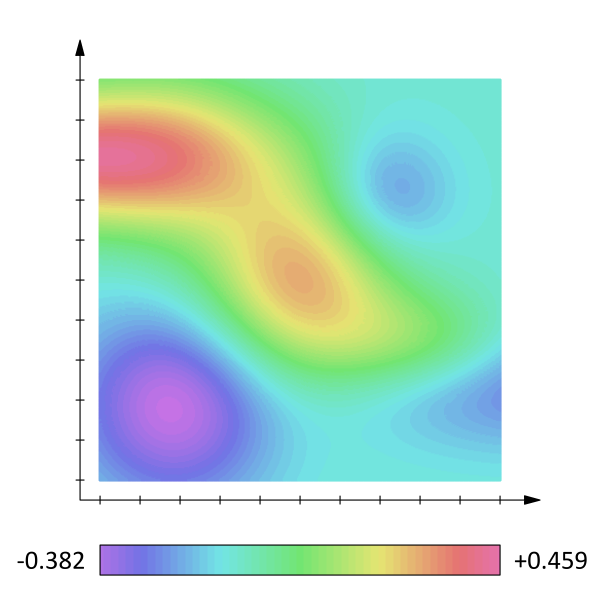
\includegraphics[width=0.7\textwidth]{Scalar_field.png} 
\caption{Scalar field,  \textit{Source: \textcircled{1}}}
\end{figure}
\end{column}
\end{columns}

} % END OF FRAME

\frame{
\frametitle{{Introduction - Vector Fields}}
\begin{columns}
\begin{column}{.5\textwidth}
\begin{itemize}
	\item Vector fields are visualized by a collection of arrows with a given magnitude and direction classically
	\bigskip
	\item Each position in space is mapped a scalar magnitude and an angle
	\bigskip
	\item Examples: flow field, magnetic field, gravitational field
\end{itemize}
\end{column}
\begin{column}{.5\textwidth}
\begin{figure}[t]
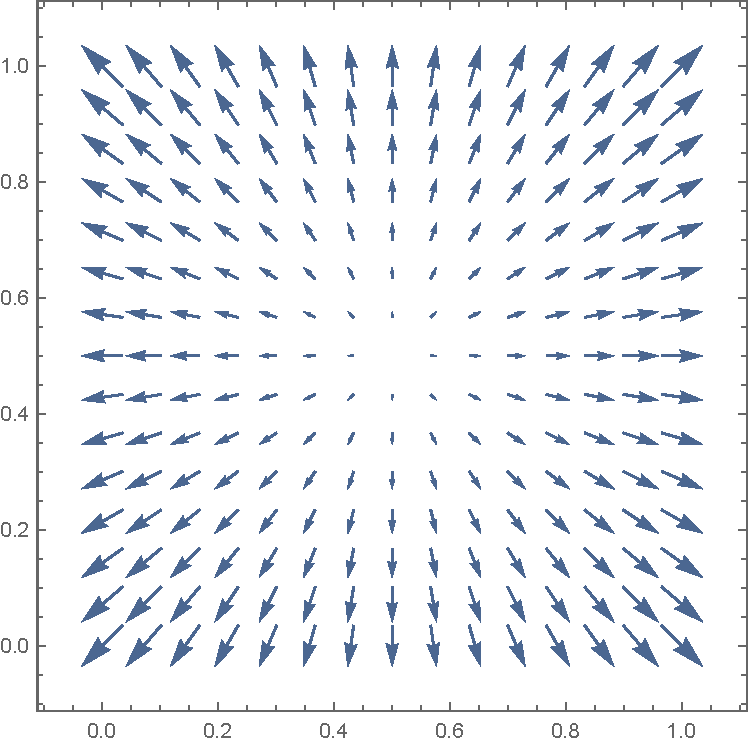
\includegraphics[width=0.6\textwidth]{vector_field.pdf} a)
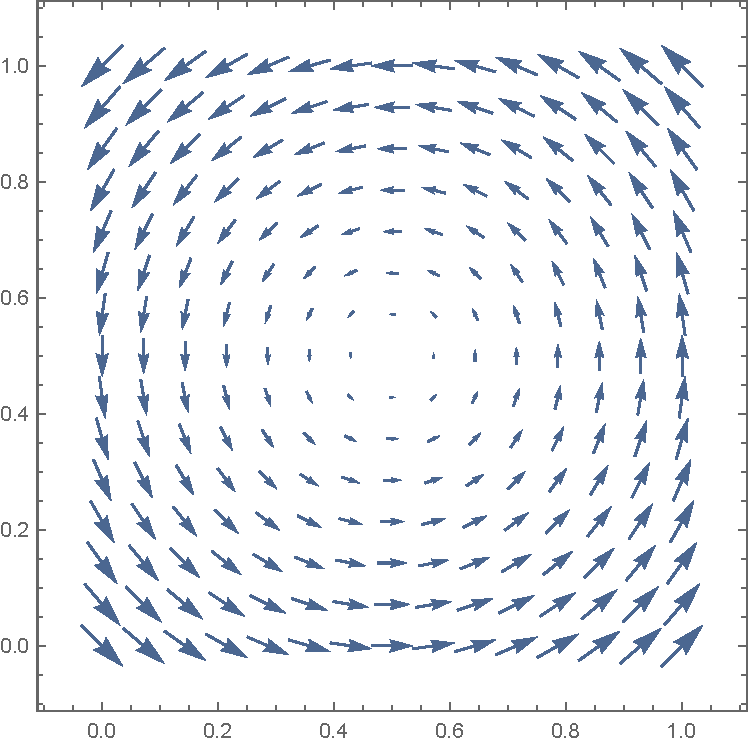
\includegraphics[width=0.6\textwidth]{vector_field2.pdf} b)
\caption{Vector fields: a) $\{x,y\}$, b) $\{-y,x\}$}
\end{figure}

\end{column}
\end{columns}

} % END OF FRAME

\frame{
\frametitle{{Introduction - Tensor Fields}}
\begin{columns}
\begin{column}{.5\textwidth}
\begin{itemize}
	\item Tensor fields are commonly visualized by:
	\begin{itemize}
		\item Glyphs
		\item Tensor field lines (TFLs) $\Rightarrow$ Hyperstreamlines
	\end{itemize}
	\bigskip
	\item Each position in space is mapped a tensor describing a directional distribution
	\bigskip
	\item Scalar Measures: anisotropy index, tensor magnitude
\end{itemize}
\end{column}
\begin{column}{.5\textwidth}
\begin{figure}[t]
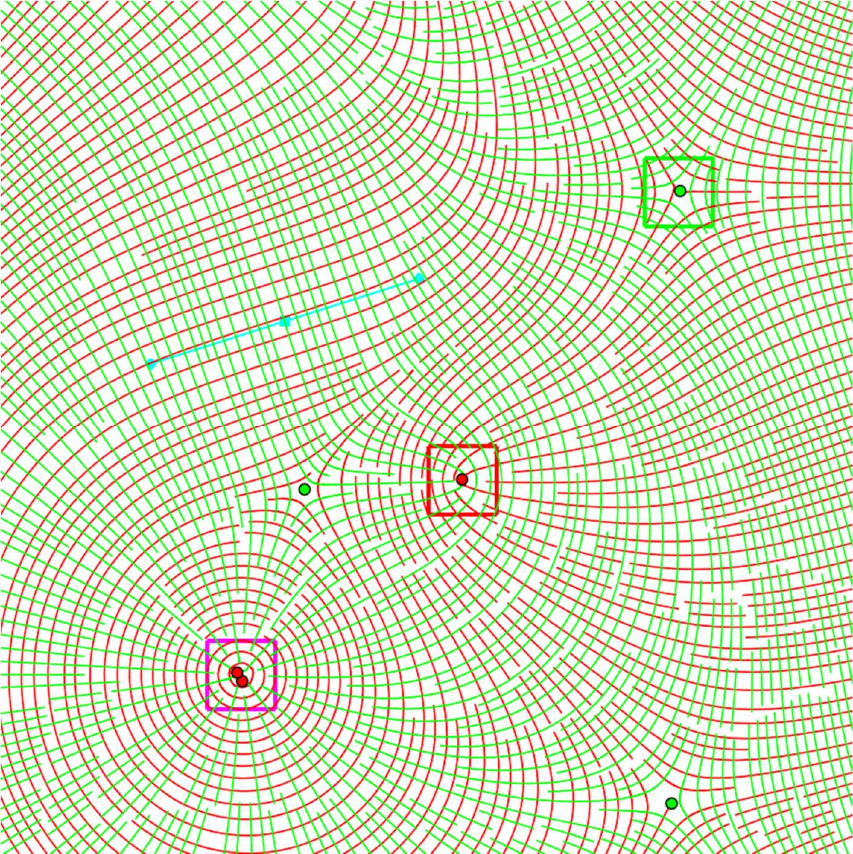
\includegraphics[width=0.6\textwidth]{hyperstreamlines.png} a)
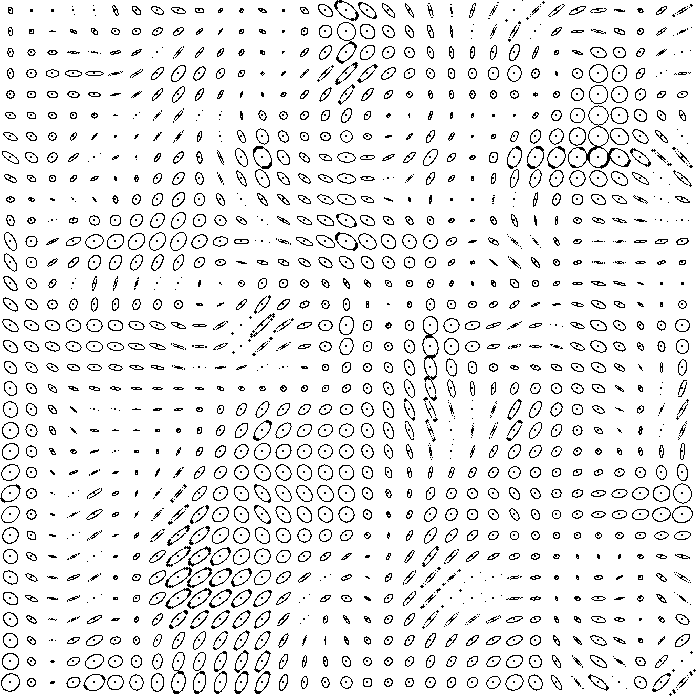
\includegraphics[width=0.6\textwidth]{random-global.png} b)
\caption{Tensor fields: a) Tensor field lines, b) Glyphs}
\end{figure}

\end{column}
\end{columns}

} % END OF FRAME

\frame{
\frametitle{{Motivation - Tensor Fields}}
\begin{figure}[!t]
\centering
  \begin{minipage}{0.3\textwidth}
      \centering
    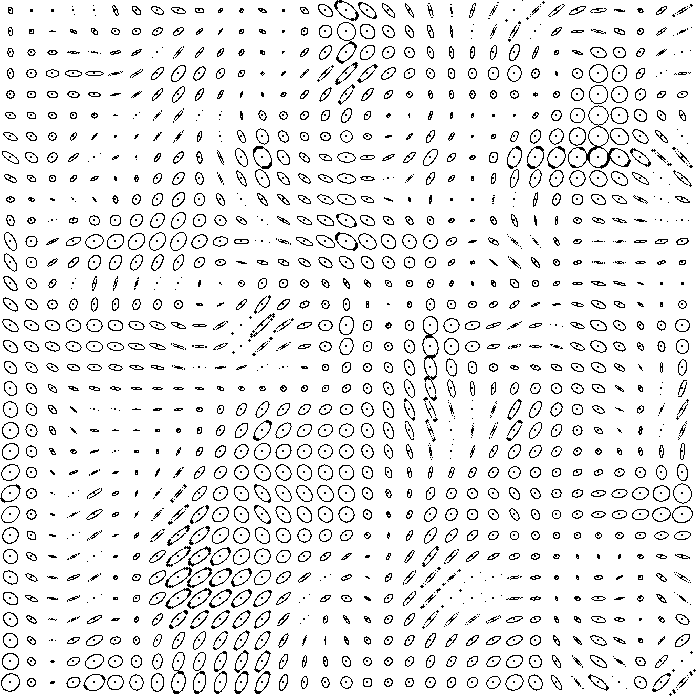
\includegraphics[height=0.7\textwidth]{random-global.png}
	a)
    \label{a)}
  \end{minipage}
  \begin{minipage}{0.3\textwidth}
      \centering
    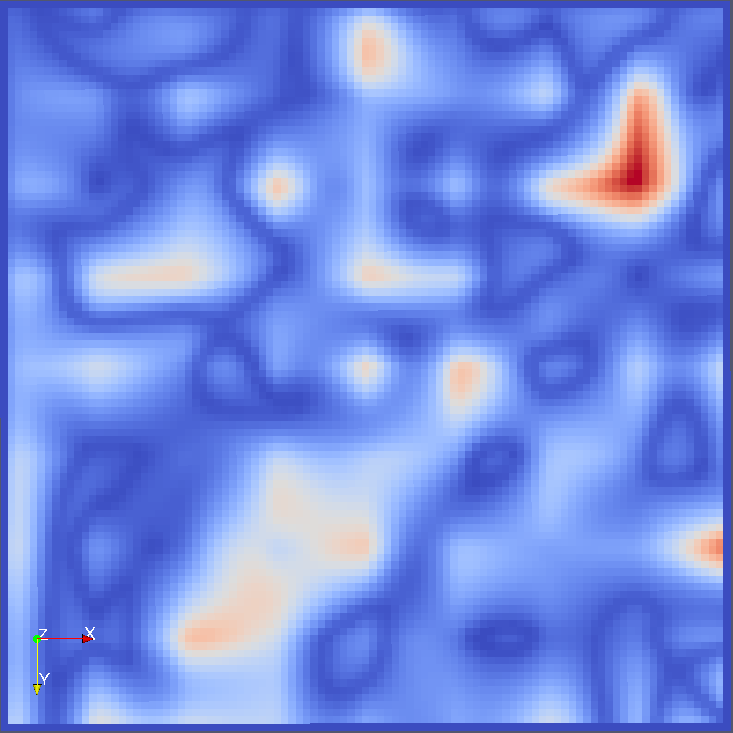
\includegraphics[height=0.7\textwidth]{random_global.png}
	b)
    \label{b)}
  \end{minipage}
  \begin{minipage}{0.3\textwidth}
      \centering
    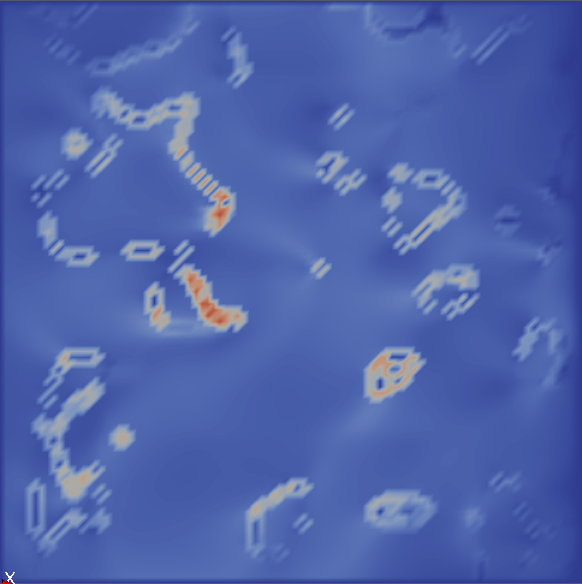
\includegraphics[height=0.7\textwidth]{random_local_slice0.png}
	c)
    \label{b)}
  \end{minipage}
\caption{Random field: a) field, b) tensor magnitude, c) FTLE}
\label{test_fields2}
\end{figure}
Applications:
\begin{itemize}
	\item Vector fields: to describe the directionally dependent spatial gradient called Jacobian-matrix,
	\item Fluid and solid continuum mechanics: to describe a whole distribution of stresses
	\item DT-MRI: diffusion tensor - magnetic resonance imaging: to describe the diffusion characteristics of water molecules within tissue
\end{itemize}
} % END OF FRAME


\frame{
\frametitle{{Random Test Field}}
\begin{columns}
\begin{column}{.5\textwidth}
\begin{itemize}
	\item Tensor fields are commonly visualized by:
	\begin{itemize}
		\item Glyphs
		\item Tensor field lines (TFLs) $\Rightarrow$ Hyperstreamlines
	\end{itemize}
	\bigskip
	\item Each position in space is mapped a tensor describing a directional distribution
	\bigskip
	\item Scalar Measures: anisotropy index, tensor magnitude
\end{itemize}
\end{column}
\begin{column}{.5\textwidth}
\begin{figure}[!t]
\centering
  \begin{minipage}{0.4\textwidth}
  \centering
    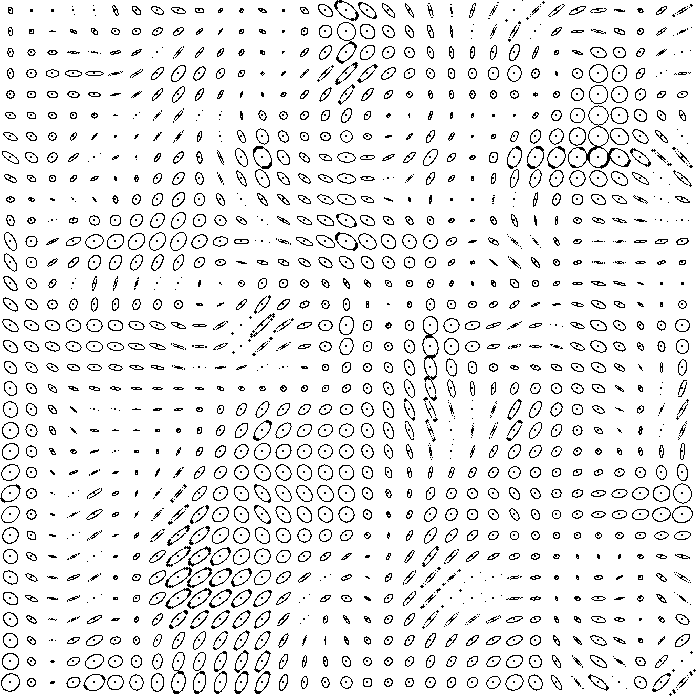
\includegraphics[width=\textwidth]{random-global.png}
	a)
  \end{minipage}
  \begin{minipage}{0.4\textwidth}
  \centering
    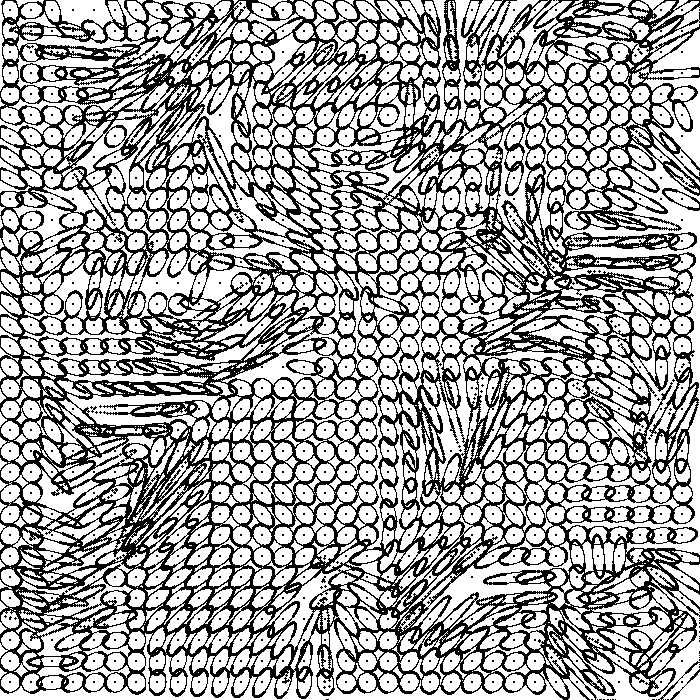
\includegraphics[width=\textwidth]{random-local.png}
	b)
  \end{minipage}
\label{bow_contour}
\end{figure}
\begin{figure}[!t]
\centering
  \begin{minipage}{0.4\textwidth}
  \centering
    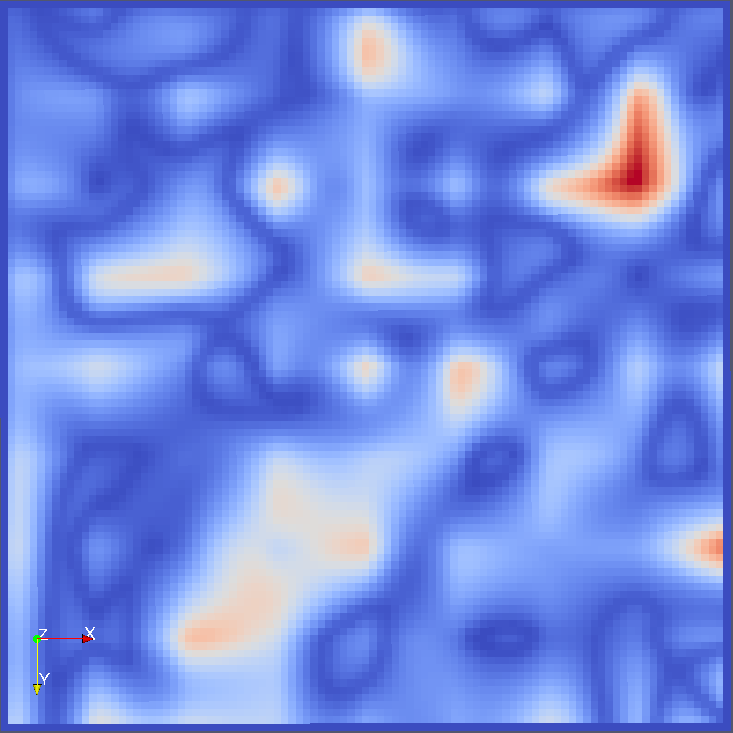
\includegraphics[width=\textwidth]{random_global.png}
	c)
  \end{minipage}
  \begin{minipage}{0.4\textwidth}
  \centering
    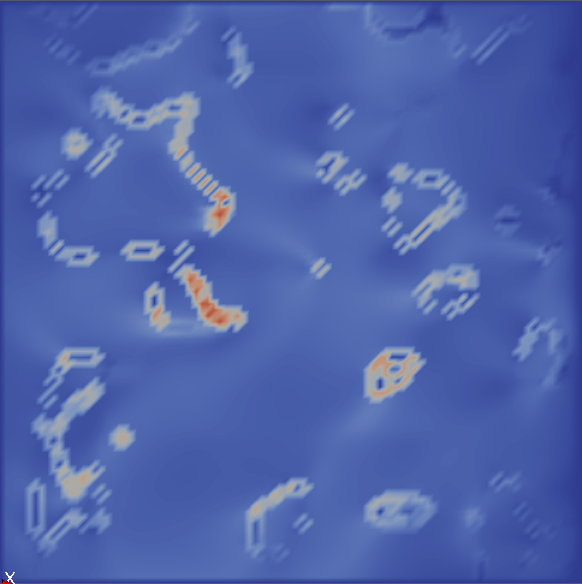
\includegraphics[width=\textwidth]{random_local_slice0.png}
	d)
  \end{minipage}
    \caption{Random test field : a) Global, b) Local normalization, c) Tensor mag. d) LTG (FTLE)}
\label{bow_contour}
\end{figure}
\end{column}
\end{columns}

} % END OF FRAME

\frame{
\frametitle{{Random Test Field - Evaluation}}
\begin{columns}
\begin{column}{.5\textwidth}
\begin{itemize}
	\item numerics: limit number representation to a particular range
	\item preposition for relatively high tensor mags.: $\lambda_1\approx\lambda_2\approx1.0$ (because ellipsoid area equals $A=\lambda_1\cdot\lambda_2\cdot\pi$)\\
\end{itemize}
\end{column}
\begin{column}{.5\textwidth}
\begin{figure}[!t]
\centering
  \begin{minipage}{0.4\textwidth}
  \centering
    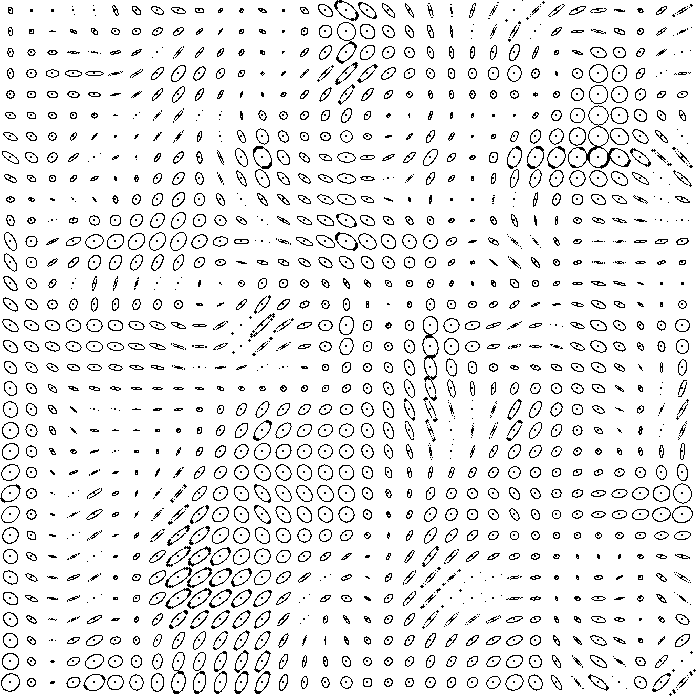
\includegraphics[width=\textwidth]{random-global.png}
	a)
  \end{minipage}
  \begin{minipage}{0.4\textwidth}
  \centering
    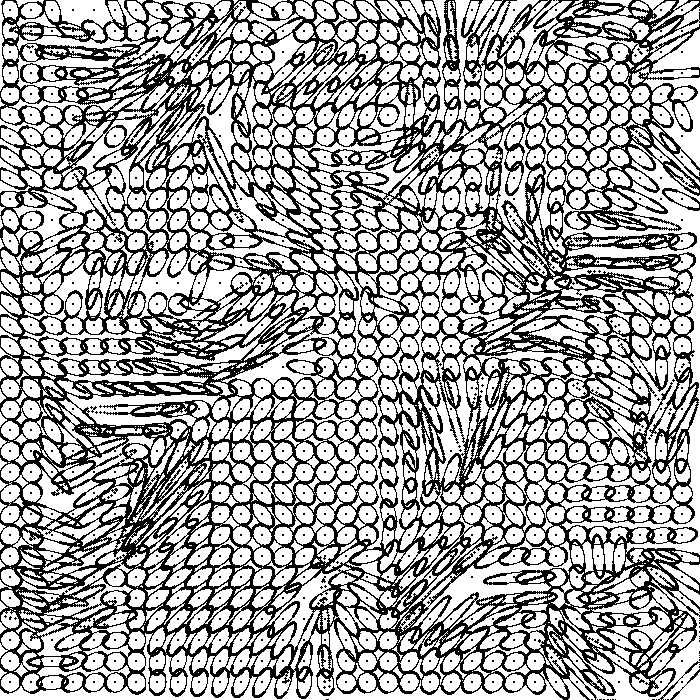
\includegraphics[width=\textwidth]{random-local.png}
	b)
  \end{minipage}
\label{bow_contour}
\end{figure}
\begin{figure}[!t]
\centering
  \begin{minipage}{0.4\textwidth}
  \centering
    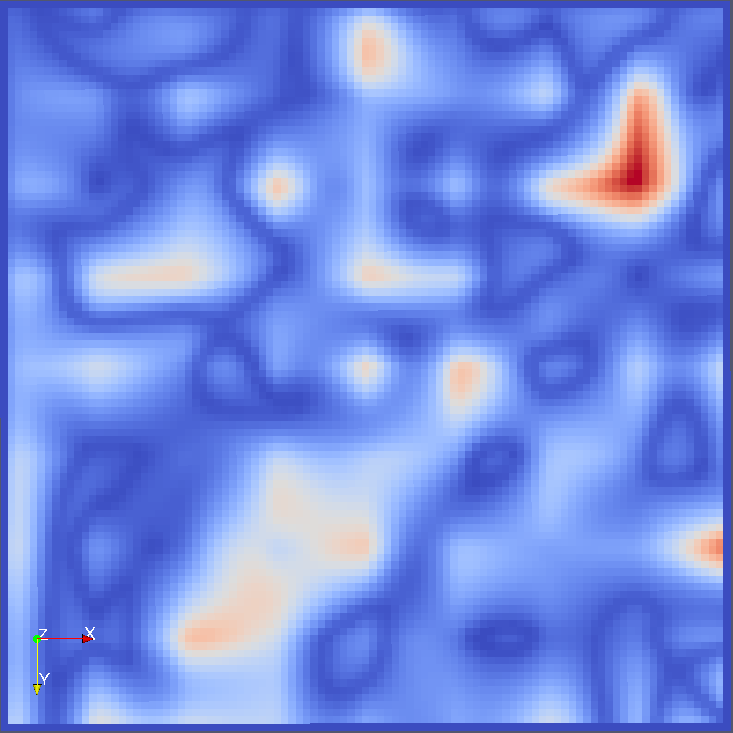
\includegraphics[width=\textwidth]{random_global.png}
	c)
  \end{minipage}
  \begin{minipage}{0.4\textwidth}
  \centering
    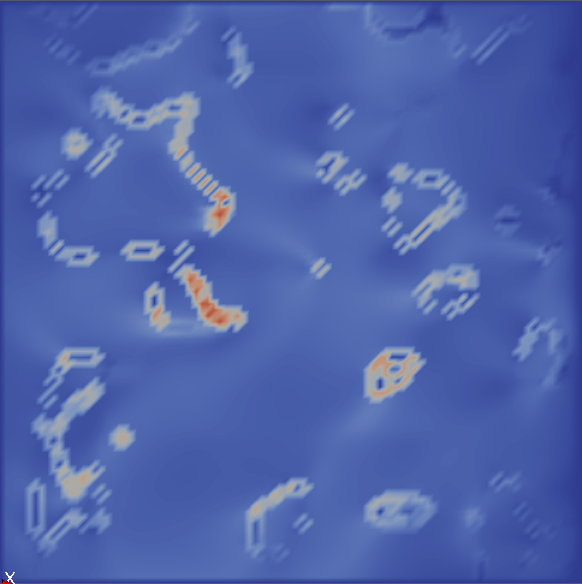
\includegraphics[width=\textwidth]{random_local_slice0.png}
	d)
  \end{minipage}
    \caption{Random test field : a) Global, b) Local normalization, c) Tensor mag. d) LTG (FTLE)}
\label{bow_contour}
\end{figure}
\end{column}
\end{columns}

%$\Rightarrow$ chances are about $50\%$ for relatively low tensor magnitudes (ellipsoid areas)
} % END OF FRAME

\frame{
\frametitle{{Heart dataset - Evaluation}}
\begin{figure}[!t]
\centering
  \begin{minipage}{0.3\textwidth}
  \centering
  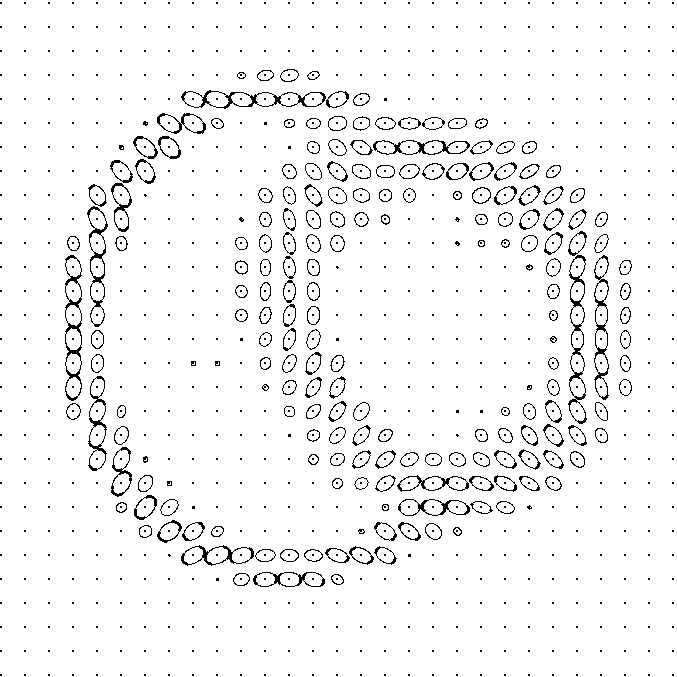
\includegraphics[width=\textwidth]{heartDwnsmpl.PNG}
	a)
    \label{a)}
  \end{minipage}
  \begin{minipage}{0.3\textwidth}
  \centering
    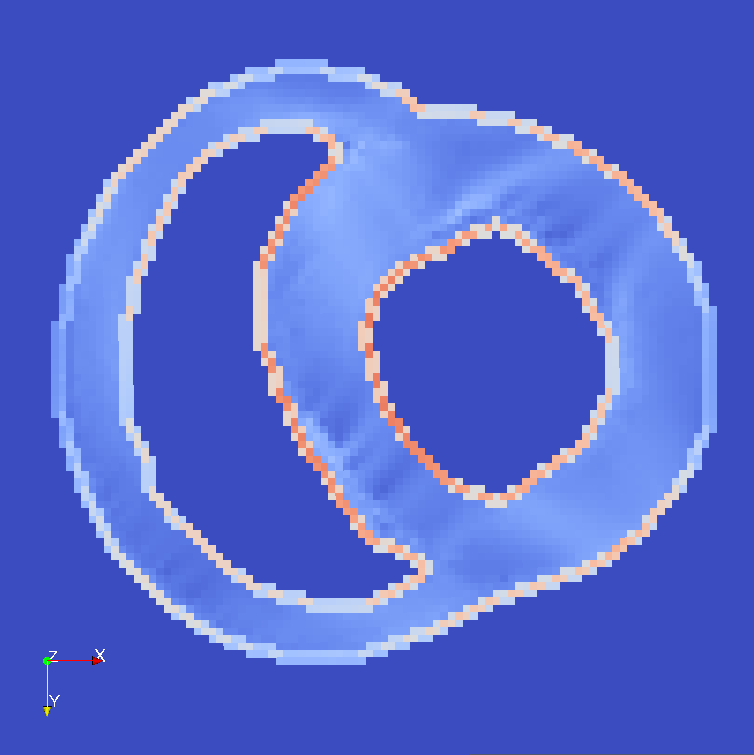
\includegraphics[width=\textwidth]{heart_slice20.PNG}
	b)
    \label{b)}
  \end{minipage}
  \begin{minipage}{0.3\textwidth}
  \centering
    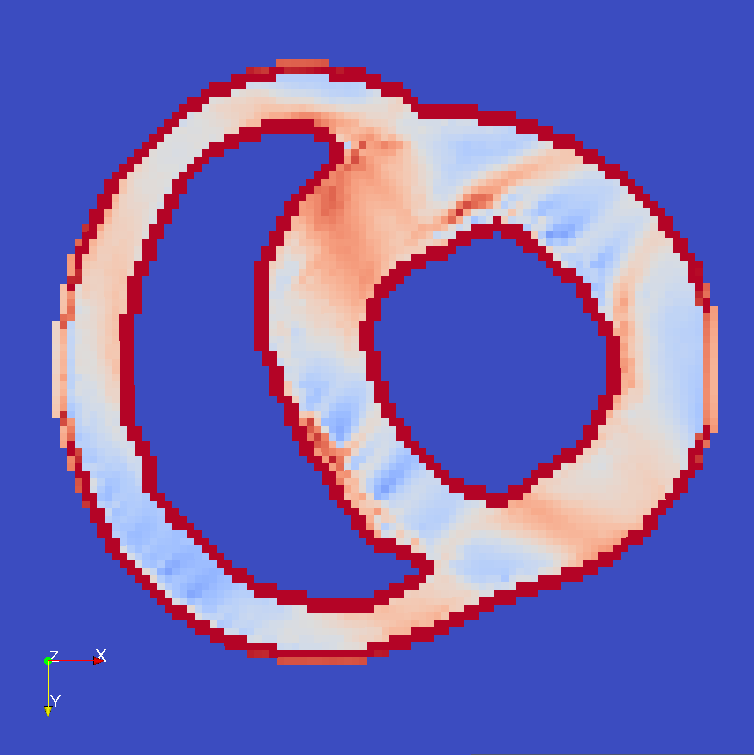
\includegraphics[width=\textwidth]{heart_slice20_rescale.PNG}
	c)
    \label{b)}
  \end{minipage}
  \caption{Heart test field: a) Glyphs, b) LTG local, c) LTG local (rescale)}
\label{heart-ftle}
\end{figure}
\begin{itemize}
	\item light ridges enhanced by rescaling for the down-left direction
	\item these regions exhibit most drastic changes in anisotropy and/or divergence for TFLs
	\item edge artifacts: edges effect high gradients for the flow map
\end{itemize}
} % END OF FRAME

\frame{
\frametitle{{Heart dataset - Evaluation}}
\begin{figure}[!t]
\centering
  \begin{minipage}{0.3\textwidth}
  \centering
  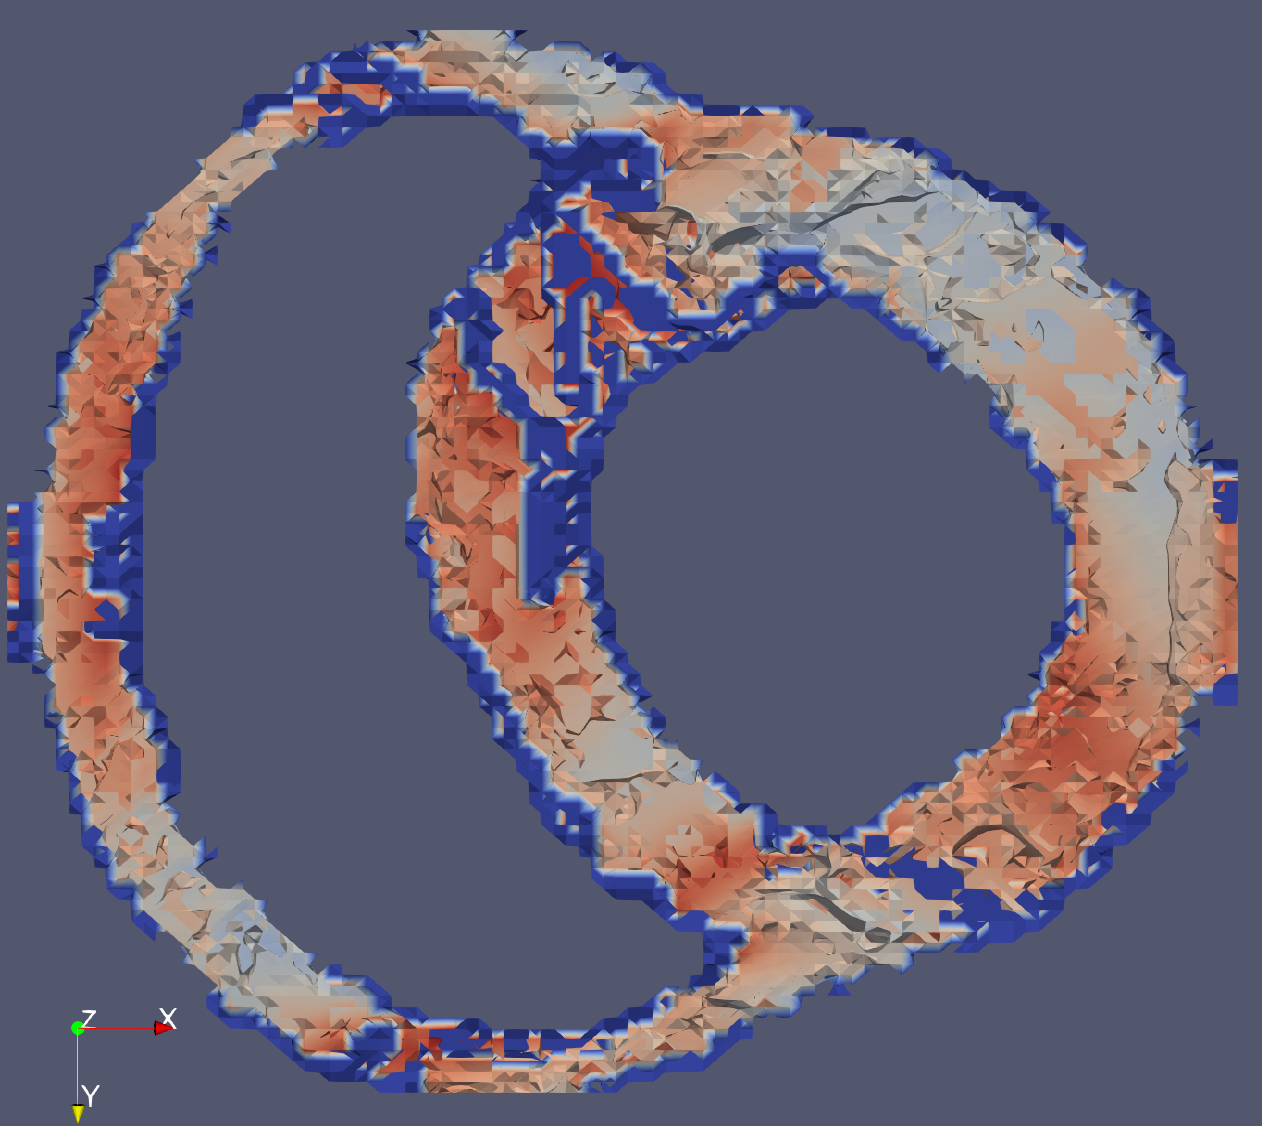
\includegraphics[width=\textwidth]{heart_vcgRidges4.PNG}
	a)
    \label{a)}
  \end{minipage}
  \begin{minipage}{0.3\textwidth}
  \centering
    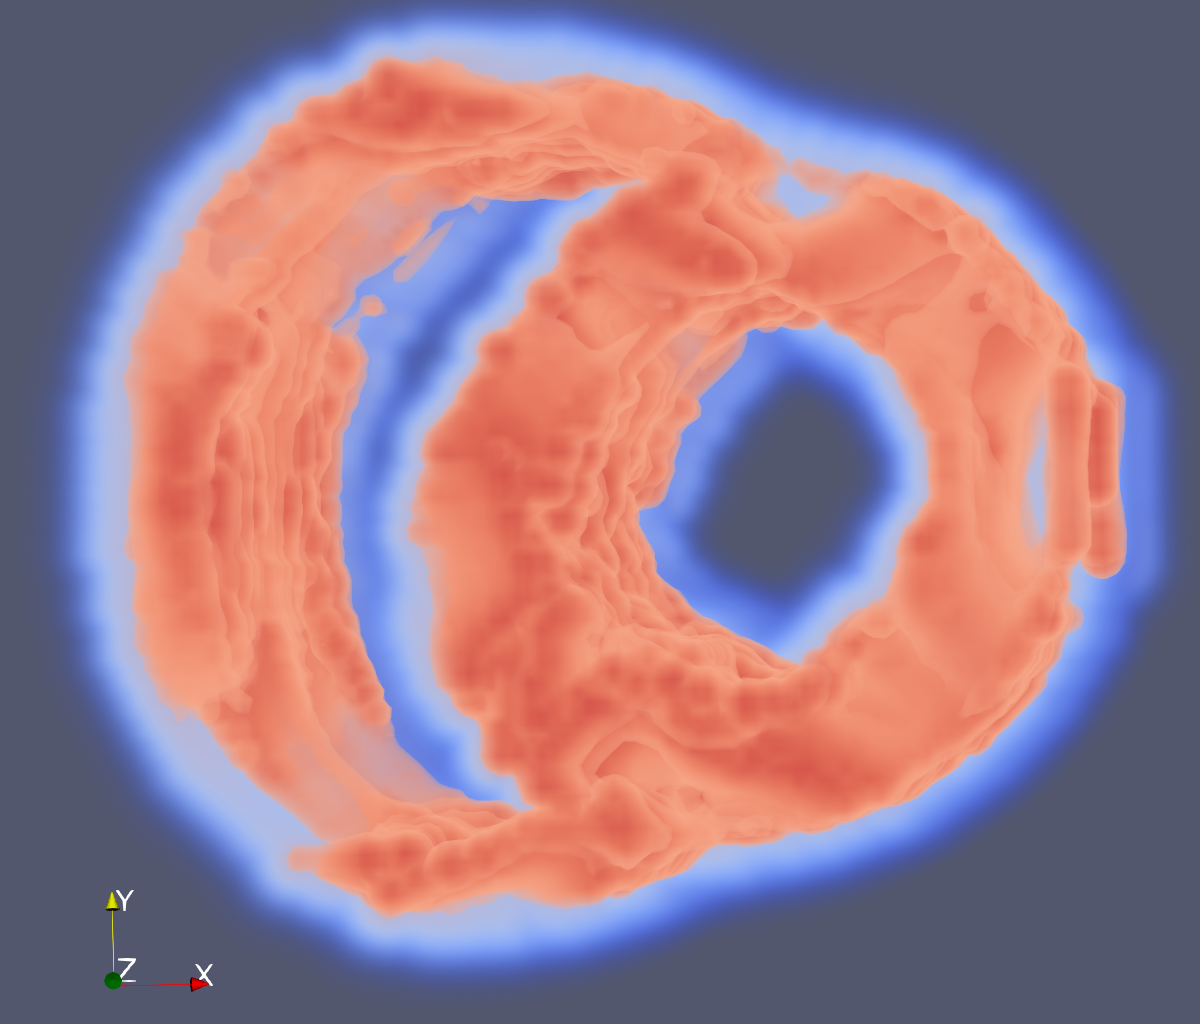
\includegraphics[width=\textwidth]{heart_isoVolume3.PNG}
	b)
    \label{b)}
  \end{minipage}
  \begin{minipage}{0.3\textwidth}
  \centering
    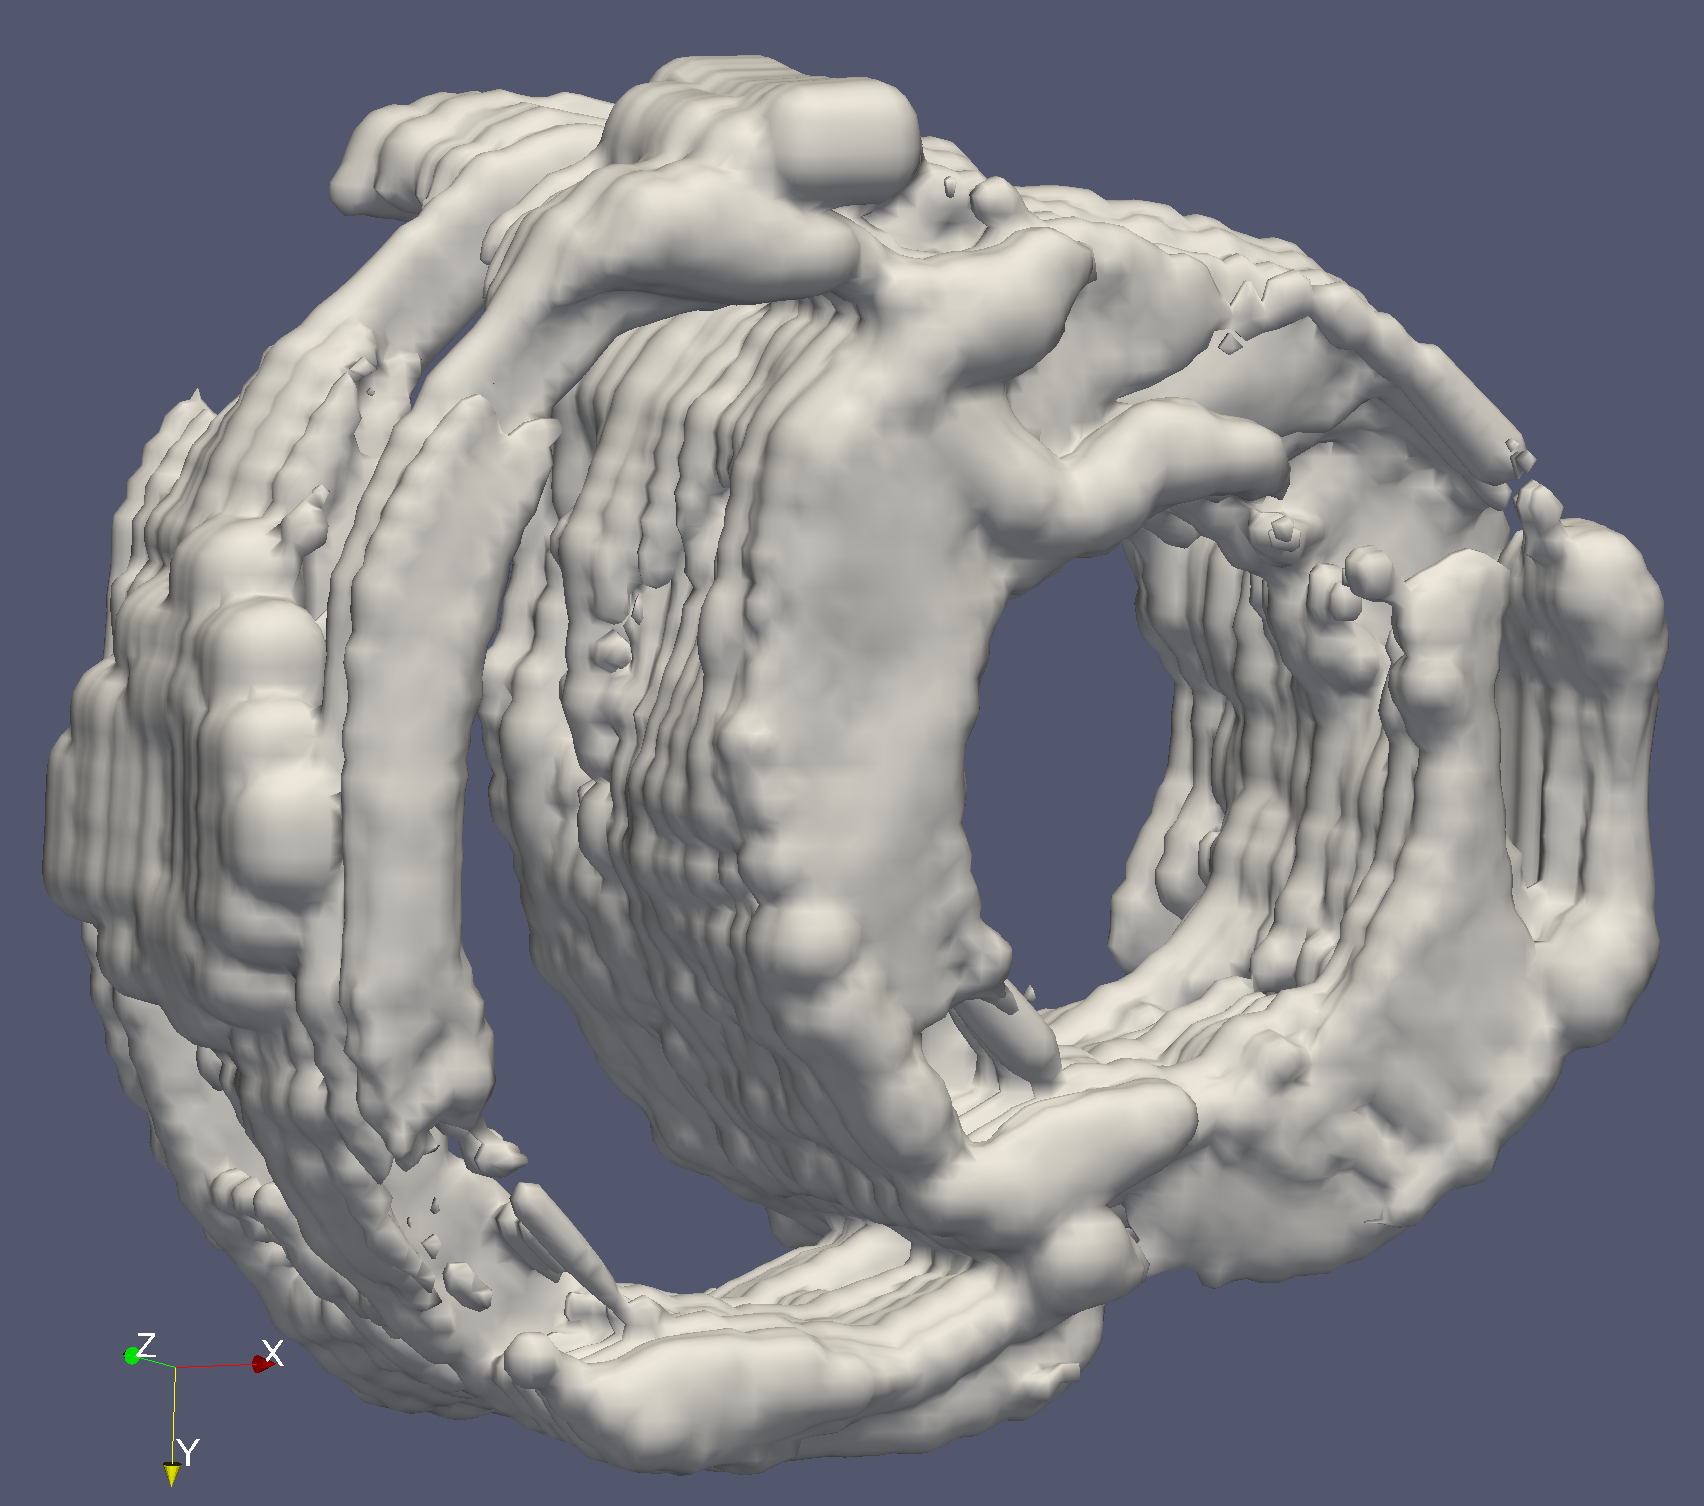
\includegraphics[width=\textwidth]{heart_contour.PNG}
	c)
    \label{b)}
  \end{minipage}
  \caption{Heart test field: a) Glyphs, b) LTG local, c) LTG local (rescale)}
\label{heart-ftle}
\end{figure}
\begin{itemize}
	\item volumes reveal blob-shaped features
	\item these features in turn form 3D ridges representing LCS
\end{itemize}
} % END OF FRAME

%%%%%%%%%%%%%%%%%%%%%%%%%%%%%%%%%%%%%%%%%%%%%%%%%%%%%%%%%%%%

% Alternative: put content in separate files
% Check the difference between including these files using \input{filename} and \include{filename} and see which one you like better
%\chapter{Einleitung}\label{intro}
%\input{introduction}
%
%\chapter{Voraussetzungen}\label{bg}
%\input{background}



\end{document}